\section{Implementation}
\label{section:implementation}
\subsection{Mobile Player}
In this section the mobile player \gls{prefab} will be discussed. 
\gls{see} is supported on multiple platforms and with each platform having different requirements each platform needs to be divided.
Therefore, each platform gets its own player \gls{prefab}.
The mobile player prefab for the \gls{android} version of \gls{see} can be seen in figure \ref{fig:prefab}.

\begin{figure}[htb]
    \centering
    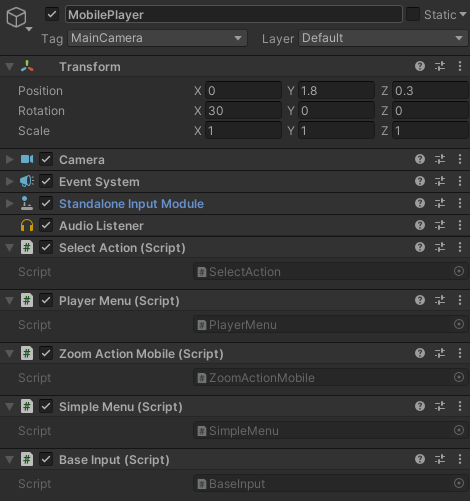
\includegraphics[width=0.8\textwidth]{Implementation/img/mobile_player.png}
    \caption{The mobile player \gls{prefab}}\label{fig:prefab}
\end{figure}

\subsubsection{PlayerMenu Script}
\subsubsection{Prefab interactions}
\subsection{Player Movement}
\subsection{Mobile Menu}
\begin{figure}[htb]
    \centering
    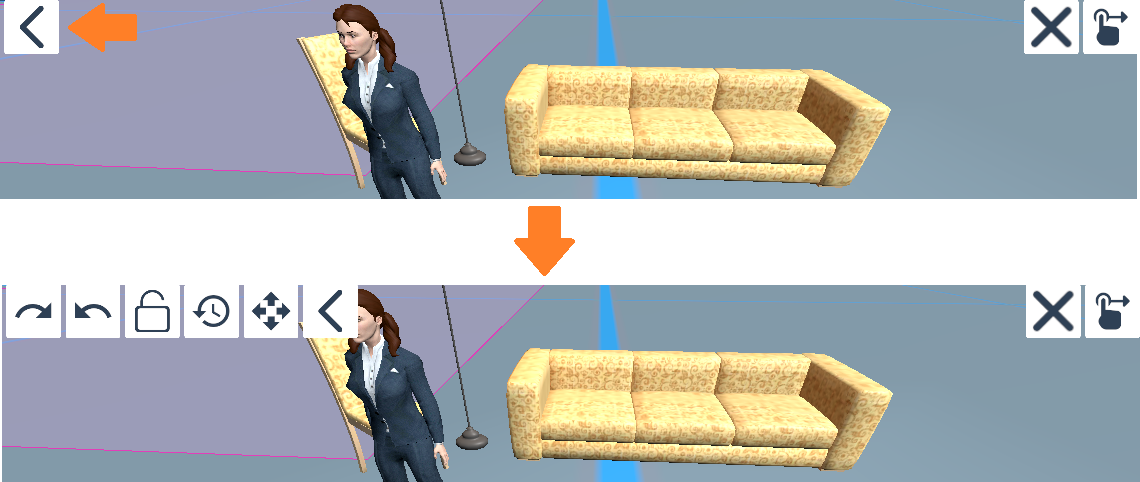
\includegraphics[width=1\textwidth]{Implementation/img/quickmenu.png}
    \caption{The \textit{quickmenu} on the left top side of the mobile device. Pressing the button with an orange marked arrow will expand the menu.}\label{fig:quickmenu}
\end{figure}

\begin{figure}[htb]
    \centering
    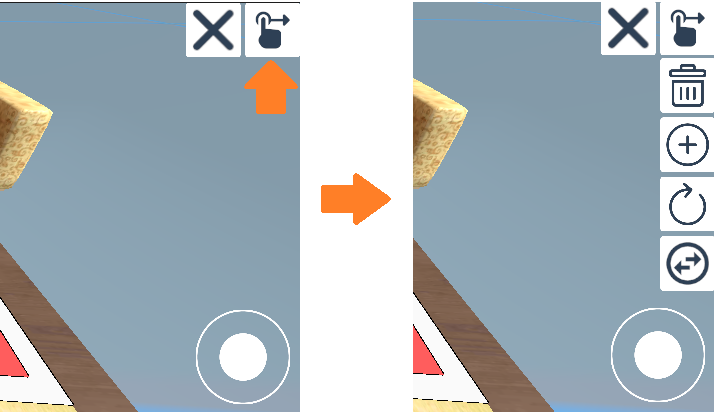
\includegraphics[width=1\textwidth]{Implementation/img/menu.png}
    \caption{The player interaction menu on the right top side of the mobile device. The button on the top right side indicate the active interaction mode. Pressing the same button also expands the menu.}\label{fig:menu}
\end{figure}